\documentclass[11pt, a4paper]{article}

% Fonts and Encoding
\usepackage[utf8]{inputenc}
\usepackage[T1]{fontenc}
\usepackage{lmodern}

% Math and Symbols
\usepackage{amsmath, amssymb, amsthm, amsfonts, mathrsfs, mathtools}

% Layout and Geometry
\usepackage{geometry}
\geometry{a4paper, margin=1in}

% Formatting and Graphics
\usepackage{graphicx, xcolor, enumitem, booktabs, array, tabularx}

% TikZ for Illustrations
\usepackage{tikz}
\usetikzlibrary{arrows.meta, positioning, shapes.geometric, calc, backgrounds, matrix}

% Clickable Links and TOC
\usepackage{hyperref}
\hypersetup{
    colorlinks=true,
    linkcolor=blue,
    filecolor=magenta,      
    urlcolor=cyan,
    pdftitle={Advanced Mathematics Topic},
}

% Theorem Environments
\newtheorem{theorem}{Theorem}[section]
\newtheorem{lemma}[theorem]{Lemma}
\newtheorem{proposition}[theorem]{Proposition}
\newtheorem{corollary}[theorem]{Corollary}
\theoremstyle{definition}
\newtheorem{definition}{Definition}[section]
\newtheorem{axiom}{Axiom}[section]
\newtheorem{example}{Example}[section]
\theoremstyle{remark}
\newtheorem{remark}{Remark}[section]

% Custom Commands (Enforced standard notation)
\newcommand{\R}{\mathbb{R}}
\newcommand{\N}{\mathbb{N}}
\newcommand{\Z}{\mathbb{Z}}
\newcommand{\Q}{\mathbb{Q}}
\newcommand{\E}{\mathbb{E}}
\newcommand{\Prob}{\mathbb{P}}
\newcommand{\F}{\mathcal{F}}

\begin{document}

\title{\textbf{Advanced Abstract Mathematics: Relations and Their Properties \\ \Large Comprehensive Practice Problem Set}}
\author{Tashfeen Omran}
\date{October 29, 2026}

\maketitle
\tableofcontents
\newpage

\section{Concept Checklist \& Question Mapping}
\label{sec:checklist_start}

This problem set is rigorously designed to test the foundational axioms, logical structures, and advanced applications of mathematical relations. Every problem maps directly to a core theoretical concept.

\vspace{1em}
\noindent
\begin{tabularx}{\textwidth}{>{\bfseries}l X l}
\toprule
ID & Concept / Technique & Problem Mapping \\
\midrule
C1 & Cartesian Products \& Basic Definitions (Domain, Range, Inverse) & 1, 2, 3, 4 \\
\addlinespace[4pt]
C2 & Reflexivity (Direct Proofs \& Counterexamples) & 5, 6 \\
\addlinespace[4pt]
C3 & Symmetry (Direct Proofs \& Counterexamples) & 7, 8, 18 \\
\addlinespace[4pt]
C4 & Transitivity (Direct Proofs \& Counterexamples) & 9, 10, 11, 21 \\
\addlinespace[4pt]
C5 & Vacuous Truth \& Edge Cases (Empty Relations, Small Sets) & 12, 13, 14, 15, 17 \\
\addlinespace[4pt]
C6 & Equivalence Relations \& Partitions & 16, 26 \\
\addlinespace[4pt]
C7 & Transitive Closure ($R^*$) \& Path Connectivity & 24, 25, 29 \\
\addlinespace[4pt]
C8 & Set-Theoretic Manipulations (Unions, Intersections, Inverses) & 19, 20, 22, 23 \\
\addlinespace[4pt]
C9 & Real-World Modeling (Bisimulation in MDPs, Arbitrage Equivalence) & 26, 27 \\
\addlinespace[4pt]
C10 & Diagnostic Testing (Finding Flaws in Logical Arguments) & 28, 29, 30 \\
\bottomrule
\end{tabularx}

\newpage

\section{Problem Set}

\subsection{Foundations: Domain, Range, and Inverses}
\textbf{Problem 1.} Let $R$ be a relation from set $A$ to set $B$. Prove rigorously that $\mathrm{dom}(R^{-1}) = \mathrm{range}(R)$.

\vspace{0.5em}
\noindent
\textbf{Problem 2.} Let $R$ be a relation from set $A$ to set $B$. Prove rigorously that $\mathrm{range}(R^{-1}) = \mathrm{dom}(R)$.

\vspace{0.5em}
\noindent
\textbf{Problem 3.} Let $R$ be a relation from set $A$ to set $B$. Prove that the inverse of the inverse relation is the original relation itself, i.e., $(R^{-1})^{-1} = R$.

\vspace{0.5em}
\noindent
\textbf{Problem 4.} Let $A$ be a finite set with $|A| = n$. Prove that the maximum number of elements in a relation $R$ on $A$ such that $R \cap R^{-1} = \emptyset$ is $\frac{n(n-1)}{2}$.

\subsection{Core Properties: Reflexivity, Symmetry, and Transitivity}
\textbf{Problem 5.} Let $R$ be a relation defined on $\Z$ by $x \ R \ y \iff x + y$ is even. Prove that $R$ is reflexive.

\vspace{0.5em}
\noindent
\textbf{Problem 6.} Let $R$ be a relation defined on $\Z$ by $x \ R \ y \iff x + y$ is odd. Prove or disprove that $R$ is reflexive.

\vspace{0.5em}
\noindent
\textbf{Problem 7.} Prove that the relation $R$ defined in Problem 5 is symmetric.

\vspace{0.5em}
\noindent
\textbf{Problem 8.} Prove that the relation $R$ defined in Problem 6 is symmetric.

\vspace{0.5em}
\noindent
\textbf{Problem 9.} Let $R$ be a relation defined on $\R$ by $x \ R \ y \iff x \cdot y \ge 0$. Prove or disprove that $R$ is transitive.

\vspace{0.5em}
\noindent
\textbf{Problem 10.} Let $R$ be a relation defined on $\N$ by $a \ R \ b \iff a \mid b \lor b \mid a$. Prove or disprove that $R$ is transitive.

\vspace{0.5em}
\noindent
\textbf{Problem 11.} Let $S$ be the set of all polynomials of degree at most 3 with real coefficients. Define a relation $R$ on $S$ by $p \ R \ q \iff p$ and $q$ share at least one real root. Prove or disprove that $R$ is transitive.

\subsection{Vacuous Truths, Edge Cases, and Counterexamples}
\textbf{Problem 12.} Let $A = \{1, 2, 3, 4\}$. Determine the maximum number of elements in a relation $R$ on $A$ such that $R$ possesses none of the following properties: reflexive, symmetric, transitive.

\vspace{0.5em}
\noindent
\textbf{Problem 13.} Let $A = \{1, 2, 3, 4\}$. Construct a relation on $A$ that is reflexive and symmetric, but not transitive.

\vspace{0.5em}
\noindent
\textbf{Problem 14.} Let $A = \{1, 2, 3, 4\}$. Construct a relation on $A$ that is reflexive and transitive, but not symmetric.

\vspace{0.5em}
\noindent
\textbf{Problem 15.} Let $A = \{1, 2, 3, 4\}$. Construct a relation on $A$ that is symmetric and transitive, but not reflexive.

\vspace{0.5em}
\noindent
\textbf{Problem 16.} Prove that if a relation $R$ on a set $A$ is symmetric and transitive, and for every $x \in A$ there exists at least one $y \in A$ such that $x \ R \ y$, then $R$ must be reflexive.

\vspace{0.5em}
\noindent
\textbf{Problem 17.} Let $R = \emptyset$ be the empty relation on a non-empty set $A = \{1\}$. Prove that $R$ is symmetric and transitive, but not reflexive.

\subsection{Set-Theoretic Manipulations of Relations}
\textbf{Problem 18.} Let $R$ be a relation on a set $A$. Prove that $R$ is symmetric if and only if $R = R^{-1}$.

\vspace{0.5em}
\noindent
\textbf{Problem 19.} Let $R_1$ and $R_2$ be relations from set $A$ to set $B$. Prove that $(R_1 \cup R_2)^{-1} = R_1^{-1} \cup R_2^{-1}$.

\vspace{0.5em}
\noindent
\textbf{Problem 20.} Let $R_1$ and $R_2$ be relations from set $A$ to set $B$. Prove that $(R_1 \cap R_2)^{-1} = R_1^{-1} \cap R_2^{-1}$.

\vspace{0.5em}
\noindent
\textbf{Problem 21.} Prove that if $R_1$ and $R_2$ are transitive relations on a set $A$, then their intersection $R_1 \cap R_2$ is also a transitive relation.

\vspace{0.5em}
\noindent
\textbf{Problem 22.} Let $R$ be an arbitrary relation on a set $A$. Prove that the relation $S = R \cup R^{-1}$ is symmetric.

\vspace{0.5em}
\noindent
\textbf{Problem 23.} Let $R$ be an arbitrary relation on a set $A$. Prove that the relation $S = R \cap R^{-1}$ is symmetric.

\subsection{Transitive Closure and Advanced Structures}
\textbf{Problem 24.} Let $A = \{1, 2, 3, 4\}$ and let $R = \{(1, 2), (2, 3), (3, 4)\}$. Find the transitive closure $R^*$.

\vspace{0.5em}
\noindent
\textbf{Problem 25.} Prove that a relation $R$ on a set $A$ is transitive if and only if its transitive closure $R^*$ is equal to $R$.

\subsection{Abstract Real-World Modeling}
\textbf{Problem 26 (Quantitative Finance).} Let $P$ be the set of all available financial portfolios. Let $\Omega$ be the set of all possible future states of the world. Let $X_p(\omega)$ denote the payoff of portfolio $p$ in state $\omega$. Define a relation $\sim$ on $P$ such that $p_1 \sim p_2 \iff X_{p_1}(\omega) = X_{p_2}(\omega)$ for all $\omega \in \Omega$. Prove that $\sim$ is an equivalence relation.

\vspace{0.5em}
\noindent
\textbf{Problem 27 (AI \& Markov Decision Processes).} Let $M = (S, A, P, R, \gamma)$ be a Markov Decision Process. Let $E$ be a bisimulation equivalence relation on the state space $S$. The optimal value function $V^*(s)$ satisfies the Bellman equation:
\[ V^*(s) = \max_{a \in A} \left( R(s,a) + \gamma \sum_{s' \in S} P(s' \mid s,a) V^*(s') \right) \]
Assume that $V^*$ is constant across equivalence classes (i.e., $V^*(s') = V^*(C)$ for all $s' \in C$, where $C \in S/E$). Prove that if $s_1 \ E \ s_2$, then $V^*(s_1) = V^*(s_2)$.

\subsection{Advanced Diagnostic Testing: "Find the Flaw"}
\textbf{Problem 28.} Find the logical flaw in the following proof: \\
\textit{Claim:} If $R$ is a relation on $A$ such that $R \cap R^{-1} = \emptyset$, then $R$ cannot be transitive. \\
\textit{Flawed Proof:} If $R$ is transitive, then $(x,y) \in R$ and $(y,z) \in R \implies (x,z) \in R$. If we let $z = x$, then $(x,y) \in R$ and $(y,x) \in R \implies (x,x) \in R$. But $(y,x) \in R$ means $(x,y) \in R^{-1}$, which implies $R \cap R^{-1} \neq \emptyset$. Thus, transitive relations must intersect their inverses. $\blacksquare$

\vspace{0.5em}
\noindent
\textbf{Problem 29.} Find the logical flaw in the following proof: \\
\textit{Claim:} The transitive closure of a symmetric relation is an equivalence relation. \\
\textit{Flawed Proof:} Let $R$ be a symmetric relation on $A$. By definition, its transitive closure $R^*$ is transitive. Because $R$ is symmetric, $R^*$ inherits this symmetry. Since $R^*$ is both symmetric and transitive, for any $x, y \in A$, if $x \ R^* \ y$, then $y \ R^* \ x$. By transitivity, $x \ R^* \ y$ and $y \ R^* \ x \implies x \ R^* \ x$. Thus, $R^*$ is reflexive, making it an equivalence relation. $\blacksquare$

\vspace{0.5em}
\noindent
\textbf{Problem 30.} Find the logical flaw in the following proof: \\
\textit{Claim:} If $R_1 \subseteq R_2$ and $R_2$ is an equivalence relation on $A$, then $R_1$ is also an equivalence relation on $A$. \\
\textit{Flawed Proof:} Since $R_2$ is an equivalence relation, it is reflexive, symmetric, and transitive. Because $R_1$ is a subset of $R_2$, all ordered pairs in $R_1$ are also in $R_2$. Therefore, the elements in $R_1$ inherit the properties of reflexivity, symmetry, and transitivity from $R_2$. Thus, $R_1$ is an equivalence relation. $\blacksquare$

\newpage

\section{Detailed Solutions}

\begin{proof}[\textbf{Solution to Problem 1}]
We must show that $\mathrm{dom}(R^{-1}) \subseteq \mathrm{range}(R)$ and $\mathrm{range}(R) \subseteq \mathrm{dom}(R^{-1})$. \\
\textbf{Part 1:} Let $x \in \mathrm{dom}(R^{-1})$. By the definition of domain, there exists some $y \in A$ such that $(x, y) \in R^{-1}$. By the definition of an inverse relation, $(x, y) \in R^{-1} \implies (y, x) \in R$. Since $x$ appears as the second coordinate in an ordered pair belonging to $R$, it follows by definition that $x \in \mathrm{range}(R)$. Thus, $\mathrm{dom}(R^{-1}) \subseteq \mathrm{range}(R)$. \\
\textbf{Part 2:} Let $x \in \mathrm{range}(R)$. By the definition of range, there exists some $y \in A$ such that $(y, x) \in R$. By the definition of an inverse relation, $(y, x) \in R \implies (x, y) \in R^{-1}$. Since $x$ appears as the first coordinate in an ordered pair belonging to $R^{-1}$, it follows that $x \in \mathrm{dom}(R^{-1})$. Thus, $\mathrm{range}(R) \subseteq \mathrm{dom}(R^{-1})$. \\
Since both subset inclusions hold, $\mathrm{dom}(R^{-1}) = \mathrm{range}(R)$.
\end{proof}

\begin{proof}[\textbf{Solution to Problem 2}]
We must show that $\mathrm{range}(R^{-1}) \subseteq \mathrm{dom}(R)$ and $\mathrm{dom}(R) \subseteq \mathrm{range}(R^{-1})$. \\
\textbf{Part 1:} Let $y \in \mathrm{range}(R^{-1})$. By definition, there exists some $x \in B$ such that $(x, y) \in R^{-1}$. By the definition of an inverse relation, $(x, y) \in R^{-1} \implies (y, x) \in R$. Since $y$ is the first coordinate of a pair in $R$, $y \in \mathrm{dom}(R)$. Thus, $\mathrm{range}(R^{-1}) \subseteq \mathrm{dom}(R)$. \\
\textbf{Part 2:} Let $y \in \mathrm{dom}(R)$. By definition, there exists some $x \in B$ such that $(y, x) \in R$. By the definition of an inverse relation, $(y, x) \in R \implies (x, y) \in R^{-1}$. Since $y$ is the second coordinate of a pair in $R^{-1}$, $y \in \mathrm{range}(R^{-1})$. Thus, $\mathrm{dom}(R) \subseteq \mathrm{range}(R^{-1})$. \\
Therefore, $\mathrm{range}(R^{-1}) = \mathrm{dom}(R)$.
\end{proof}

\begin{proof}[\textbf{Solution to Problem 3}]
Let $(x, y)$ be an arbitrary ordered pair. We evaluate the logical equivalences:
\begin{align*}
(x, y) \in (R^{-1})^{-1} &\iff (y, x) \in R^{-1} \quad \text{(by definition of the outer inverse)} \\ \relax
&\iff (x, y) \in R \quad \text{(by definition of the inner inverse)}
\end{align*}
Since $(x, y) \in (R^{-1})^{-1}$ if and only if $(x, y) \in R$, the two sets of ordered pairs are identical. Thus, $(R^{-1})^{-1} = R$.
\end{proof}

\begin{proof}[\textbf{Solution to Problem 4}]
The condition $R \cap R^{-1} = \emptyset$ implies that if $(x, y) \in R$, then $(y, x) \notin R$. \\
First, consider the diagonal elements $(x, x)$ for any $x \in A$. If $(x, x) \in R$, then its inverse $(x, x)$ is also in $R^{-1}$, meaning $(x, x) \in R \cap R^{-1}$, which violates the empty intersection condition. Thus, $R$ can contain exactly $0$ of the $n$ diagonal elements. \\
Second, consider the off-diagonal elements. For any pair of distinct elements $x, y \in A$ (where $x \neq y$), the relation $R$ can contain at most one of the ordered pairs $(x, y)$ or $(y, x)$. The total number of distinct ordered pairs $(x, y)$ with $x \neq y$ in $A \times A$ is $n^2 - n = n(n-1)$. \\
These pairs can be grouped into mutually exclusive sets of size 2: $\{(x, y), (y, x)\}$. There are exactly $\frac{n(n-1)}{2}$ such sets. To maximize $|R|$ while satisfying the condition, we select exactly one ordered pair from each of these sets. \\
Therefore, the maximum number of elements in $R$ is $\frac{n(n-1)}{2}$.
\end{proof}

\begin{proof}[\textbf{Solution to Problem 5}]
To prove $R$ is reflexive, we must show that for all $x \in \Z$, $x \ R \ x$. \\
Let $x \in \Z$. We evaluate the condition: $x + x = 2x$. \\
Since $x$ is an integer, $2x$ is an integer multiple of 2, which is the definition of an even number. Thus, $x + x$ is even, which implies $x \ R \ x$. Therefore, $R$ is reflexive.
\end{proof}

\begin{proof}[\textbf{Solution to Problem 6}]
We will disprove that $R$ is reflexive by providing a counterexample. \\
Let $x = 1 \in \Z$. For $R$ to be reflexive, we must have $1 \ R \ 1$. \\
Evaluating the condition: $1 + 1 = 2$. \\
Since 2 is an even number, it is not odd. Therefore, $1 \ R \ 1$ is false. Because there exists at least one element $x \in \Z$ such that $(x, x) \notin R$, the relation $R$ is not reflexive.
\end{proof}

\begin{proof}[\textbf{Solution to Problem 7}]
To prove $R$ is symmetric, we must show that for all $x, y \in \Z$, if $x \ R \ y$, then $y \ R \ x$. \\
Assume $x \ R \ y$. By definition, $x + y$ is even. \\
By the commutative property of addition over the integers, $y + x = x + y$. \\
Since $x + y$ is even, $y + x$ is also even. This implies $y \ R \ x$. \\
Therefore, $R$ is symmetric.
\end{proof}

\begin{proof}[\textbf{Solution to Problem 8}]
To prove $R$ is symmetric, we must show that for all $x, y \in \Z$, if $x \ R \ y$, then $y \ R \ x$. \\
Assume $x \ R \ y$. By definition, $x + y$ is odd. \\
By the commutative property of addition, $y + x = x + y$. \\
Since $x + y$ is odd, $y + x$ is also odd. This implies $y \ R \ x$. \\
Therefore, $R$ is symmetric.
\end{proof}

\begin{proof}[\textbf{Solution to Problem 9}]
We will disprove transitivity by providing a counterexample. \\
Let $x = -1$, $y = 0$, and $z = 1$. \\
First, check $x \ R \ y$: $x \cdot y = (-1)(0) = 0$. Since $0 \ge 0$, $x \ R \ y$ holds. \\
Second, check $y \ R \ z$: $y \cdot z = (0)(1) = 0$. Since $0 \ge 0$, $y \ R \ z$ holds. \\
Finally, check $x \ R \ z$: $x \cdot z = (-1)(1) = -1$. Since $-1 \not\ge 0$, $x \ R \ z$ is false. \\
Because we found a chain $x \ R \ y$ and $y \ R \ z$ that does not result in $x \ R \ z$, the relation $R$ is not transitive.
\end{proof}

\begin{proof}[\textbf{Solution to Problem 10}]
We will disprove transitivity by providing a counterexample. \\
Let $a = 2$, $b = 6$, and $c = 3$. \\
First, check $a \ R \ b$: Since $2 \mid 6$ is true, the disjunction $2 \mid 6 \lor 6 \mid 2$ is true. Thus, $2 \ R \ 6$. \\
Second, check $b \ R \ c$: Since $3 \mid 6$ is true, the disjunction $6 \mid 3 \lor 3 \mid 6$ is true. Thus, $6 \ R \ 3$. \\
Finally, check $a \ R \ c$: We evaluate $2 \mid 3 \lor 3 \mid 2$. Since 2 does not divide 3 evenly, and 3 does not divide 2 evenly, the disjunction is false. Thus, $2 \not R \ 3$. \\
Since $2 \ R \ 6$ and $6 \ R \ 3$ but $2 \not R \ 3$, the relation $R$ is not transitive.
\end{proof}

\begin{proof}[\textbf{Solution to Problem 11}]
We will disprove transitivity by providing a counterexample. \\
Let $p(x) = x(x-1)$, $q(x) = (x-1)(x-2)$, and $r(x) = (x-2)(x-3)$. \\
The roots of $p$ are $\{0, 1\}$. The roots of $q$ are $\{1, 2\}$. The roots of $r$ are $\{2, 3\}$. \\
Since $p$ and $q$ share the root $x = 1$, $p \ R \ q$. \\
Since $q$ and $r$ share the root $x = 2$, $q \ R \ r$. \\
However, $p$ and $r$ share no roots ($\{0, 1\} \cap \{2, 3\} = \emptyset$). Thus, $p \not R \ r$. \\
Therefore, $R$ is not transitive.
\end{proof}

\begin{proof}[\textbf{Solution to Problem 12}]
The maximum possible number of elements in $A \times A$ is $4 \times 4 = 16$. We want to maximize $|R|$ by removing the minimum number of elements to break all three properties. \\
1. \textbf{Break Reflexivity:} We must remove at least one diagonal element. Let us remove $(4, 4)$. \\
2. \textbf{Break Symmetry:} We must have a pair where $(x, y) \in R$ but $(y, x) \notin R$. This requires removing at least one off-diagonal element. Let us remove $(2, 1)$ while keeping $(1, 2)$. \\
Currently, we have removed 2 elements, leaving $|R| = 14$. \\
3. \textbf{Check Transitivity:} We must verify if this 14-element relation is transitive. Notice that $(2, 3) \in R$ and $(3, 1) \in R$ (since we only removed $(4,4)$ and $(2,1)$). If $R$ were transitive, we would require $(2, 1) \in R$. However, we explicitly removed $(2, 1)$. Thus, $R$ is automatically not transitive. \\
Since we successfully broke all three properties by removing exactly 2 elements, the maximum number of elements is $16 - 2 = 14$.
\end{proof}

\begin{proof}[\textbf{Solution to Problem 13}]
Let $\Delta = \{(1,1), (2,2), (3,3), (4,4)\}$ represent the reflexive baseline. \\
Let $R = \Delta \cup \{(1, 2), (2, 1), (2, 3), (3, 2)\}$. \\
- \textbf{Reflexive:} Yes, $\Delta \subseteq R$. \\
- \textbf{Symmetric:} Yes, every off-diagonal pair has its mirror. \\
- \textbf{Transitive (Failed):} We have $(1, 2) \in R$ and $(2, 3) \in R$, but $(1, 3) \notin R$.
\end{proof}

\begin{proof}[\textbf{Solution to Problem 14}]
Let $\Delta = \{(1,1), (2,2), (3,3), (4,4)\}$. \\
Let $R = \Delta \cup \{(1, 2)\}$. \\
- \textbf{Reflexive:} Yes, $\Delta \subseteq R$. \\
- \textbf{Transitive:} Yes, the only chains of length 2 involving distinct elements are $(1,1) \to (1,2)$ and $(1,2) \to (2,2)$, both of which yield $(1,2) \in R$. \\
- \textbf{Symmetric (Failed):} We have $(1, 2) \in R$, but $(2, 1) \notin R$.
\end{proof}

\begin{proof}[\textbf{Solution to Problem 15}]
Let $R = \{(1, 1)\}$. \\
- \textbf{Symmetric:} Yes, $(1, 1)$ is its own mirror. \\
- \textbf{Transitive:} Yes, the only chain is $(1, 1)$ and $(1, 1) \implies (1, 1) \in R$. \\
- \textbf{Reflexive (Failed):} The elements $2, 3, 4 \in A$, but $(2, 2) \notin R$.
\end{proof}

\begin{proof}[\textbf{Solution to Problem 16}]
Let $x \in A$ be an arbitrary element. We must show $(x, x) \in R$. \\
By the premise, for every $x \in A$, there exists some $y \in A$ such that $(x, y) \in R$. \\
Since $R$ is symmetric, $(x, y) \in R \implies (y, x) \in R$. \\
Since $R$ is transitive, the chain $(x, y) \in R$ and $(y, x) \in R$ implies that $(x, x) \in R$. \\
Because this holds for all $x \in A$, the relation $R$ is reflexive.
\end{proof}

\begin{proof}[\textbf{Solution to Problem 17}]
- \textbf{Symmetric:} The condition for symmetry is $\forall x, y \in A, (x, y) \in R \implies (y, x) \in R$. Since $R = \emptyset$, the premise $(x, y) \in R$ is always false. Thus, the implication is vacuously true. \\
- \textbf{Transitive:} The condition is $\forall x, y, z \in A, (x, y) \in R \land (y, z) \in R \implies (x, z) \in R$. The premise is always false, making the implication vacuously true. \\
- \textbf{Reflexive:} The condition is $\forall x \in A, (x, x) \in R$. Since $A = \{1\}$, we must have $(1, 1) \in R$. But $R = \emptyset$, so $(1, 1) \notin R$. Thus, $R$ is not reflexive.
\end{proof}

\begin{proof}[\textbf{Solution to Problem 18}]
We must prove both directions of the biconditional. \\
\textbf{Forward ($\implies$):} Assume $R$ is symmetric. Let $(x, y) \in R$. By symmetry, $(y, x) \in R$. By definition of inverse, $(y, x) \in R \implies (x, y) \in R^{-1}$. Thus $R \subseteq R^{-1}$. Now let $(a, b) \in R^{-1}$. By definition, $(b, a) \in R$. By symmetry, $(a, b) \in R$. Thus $R^{-1} \subseteq R$. Therefore, $R = R^{-1}$. \\
\textbf{Backward ($\impliedby$):} Assume $R = R^{-1}$. Let $(x, y) \in R$. Since $R = R^{-1}$, $(x, y) \in R^{-1}$. By definition of inverse, this implies $(y, x) \in R$. Thus, for any $(x, y) \in R$, $(y, x) \in R$, which is the exact definition of symmetry.
\end{proof}

\begin{proof}[\textbf{Solution to Problem 19}]
Let $(x, y)$ be an arbitrary ordered pair. We evaluate the logical equivalences:
\begin{align*}
(x, y) \in (R_1 \cup R_2)^{-1} &\iff (y, x) \in (R_1 \cup R_2) \quad \text{(by definition of inverse)} \\ \relax
&\iff (y, x) \in R_1 \lor (y, x) \in R_2 \quad \text{(by definition of union)} \\ \relax
&\iff (x, y) \in R_1^{-1} \lor (x, y) \in R_2^{-1} \quad \text{(by definition of inverse)} \\ \relax
&\iff (x, y) \in (R_1^{-1} \cup R_2^{-1}) \quad \text{(by definition of union)}
\end{align*}
Since the logical statements are equivalent, the sets are identical.
\end{proof}

\begin{proof}[\textbf{Solution to Problem 20}]
Let $(x, y)$ be an arbitrary ordered pair. We evaluate the logical equivalences:
\begin{align*}
(x, y) \in (R_1 \cap R_2)^{-1} &\iff (y, x) \in (R_1 \cap R_2) \quad \text{(by definition of inverse)} \\ \relax
&\iff (y, x) \in R_1 \land (y, x) \in R_2 \quad \text{(by definition of intersection)} \\ \relax
&\iff (x, y) \in R_1^{-1} \land (x, y) \in R_2^{-1} \quad \text{(by definition of inverse)} \\ \relax
&\iff (x, y) \in (R_1^{-1} \cap R_2^{-1}) \quad \text{(by definition of intersection)}
\end{align*}
Since the logical statements are equivalent, the sets are identical.
\end{proof}

\begin{proof}[\textbf{Solution to Problem 21}]
Assume $R_1$ and $R_2$ are transitive. We must show that if $(x, y) \in R_1 \cap R_2$ and $(y, z) \in R_1 \cap R_2$, then $(x, z) \in R_1 \cap R_2$. \\
By definition of intersection, $(x, y) \in R_1 \cap R_2 \implies (x, y) \in R_1$ and $(x, y) \in R_2$. \\
Similarly, $(y, z) \in R_1 \cap R_2 \implies (y, z) \in R_1$ and $(y, z) \in R_2$. \\
Since $R_1$ is transitive, $(x, y) \in R_1$ and $(y, z) \in R_1 \implies (x, z) \in R_1$. \\
Since $R_2$ is transitive, $(x, y) \in R_2$ and $(y, z) \in R_2 \implies (x, z) \in R_2$. \\
Because $(x, z) \in R_1$ and $(x, z) \in R_2$, it follows that $(x, z) \in R_1 \cap R_2$. Thus, the intersection is transitive.
\end{proof}

\begin{proof}[\textbf{Solution to Problem 22}]
Let $S = R \cup R^{-1}$. To prove $S$ is symmetric, we must show $S = S^{-1}$. \\
Using the property from Problem 19, we have:
\[ S^{-1} = (R \cup R^{-1})^{-1} = R^{-1} \cup (R^{-1})^{-1} \]
Using the property from Problem 3, $(R^{-1})^{-1} = R$. Thus:
\[ S^{-1} = R^{-1} \cup R \]
By the commutative property of set union, $R^{-1} \cup R = R \cup R^{-1} = S$. \\
Since $S = S^{-1}$, the relation $S$ is symmetric.
\end{proof}

\begin{proof}[\textbf{Solution to Problem 23}]
Let $S = R \cap R^{-1}$. To prove $S$ is symmetric, we must show $S = S^{-1}$. \\
Using the property from Problem 20, we have:
\[ S^{-1} = (R \cap R^{-1})^{-1} = R^{-1} \cap (R^{-1})^{-1} \]
Using the property from Problem 3, $(R^{-1})^{-1} = R$. Thus:
\[ S^{-1} = R^{-1} \cap R \]
By the commutative property of set intersection, $R^{-1} \cap R = R \cap R^{-1} = S$. \\
Since $S = S^{-1}$, the relation $S$ is symmetric.
\end{proof}

\begin{proof}[\textbf{Solution to Problem 24}]
The transitive closure $R^*$ is the smallest transitive relation containing $R$. We systematically add all pairs reachable via intermediate steps. \\
- \textbf{Paths of length 1 (Original $R$):} $(1, 2), (2, 3), (3, 4)$ \\
- \textbf{Paths of length 2:} Since $1 \to 2 \to 3$, we add $(1, 3)$. Since $2 \to 3 \to 4$, we add $(2, 4)$. \\
- \textbf{Paths of length 3:} Since $1 \to 2 \to 3 \to 4$, we add $(1, 4)$. \\
Thus, $R^* = \{(1, 2), (2, 3), (3, 4), (1, 3), (2, 4), (1, 4)\}$.

\begin{center}
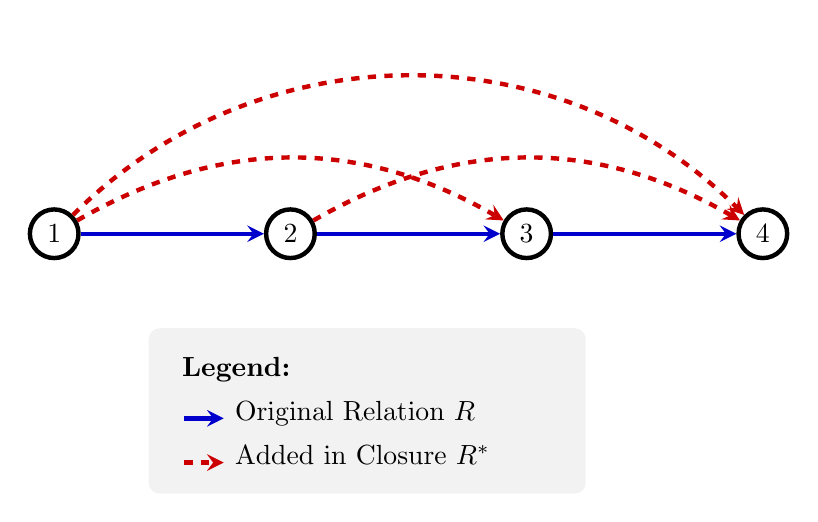
\begin{tikzpicture}[scale=1.5]
    % Background for Legend
    \fill[gray!10, rounded corners] (0.8, -2.2) rectangle (4.5, -0.8);
    
    % Nodes
    \node[draw, circle, ultra thick, black] (1) at (0,0) {$1$};
    \node[draw, circle, ultra thick, black] (2) at (2,0) {$2$};
    \node[draw, circle, ultra thick, black] (3) at (4,0) {$3$};
    \node[draw, circle, ultra thick, black] (4) at (6,0) {$4$};
    
    % Original Edges
    \draw[->, >=stealth, ultra thick, blue!80!black] (1) -- (2);
    \draw[->, >=stealth, ultra thick, blue!80!black] (2) -- (3);
    \draw[->, >=stealth, ultra thick, blue!80!black] (3) -- (4);
    
    % Closure Edges
    \draw[->, >=stealth, ultra thick, red!80!black, dashed] (1) to[bend left=30] (3);
    \draw[->, >=stealth, ultra thick, red!80!black, dashed] (2) to[bend left=30] (4);
    \draw[->, >=stealth, ultra thick, red!80!black, dashed] (1) to[bend left=45] (4);
    
    % Legend
    \node[align=left, anchor=west, black] at (1, -1.5) {
        \textbf{Legend:} \\[4pt]
        \tikz{\draw[->, >=stealth, ultra thick, blue!80!black] (0,0) -- (0.5,0);} Original Relation $R$ \\[4pt]
        \tikz{\draw[->, >=stealth, ultra thick, red!80!black, dashed] (0,0) -- (0.5,0);} Added in Closure $R^*$
    };
\end{tikzpicture}
\end{center}
\end{proof}

\begin{proof}[\textbf{Solution to Problem 25}]
We must prove both directions. \\
\textbf{Forward ($\implies$):} Assume $R$ is transitive. By definition, $R^*$ is the intersection of all transitive relations containing $R$. Since $R$ is itself a transitive relation containing $R$, it is one of the sets in the intersection. The intersection of a collection of sets containing $R$ must be a subset of $R$. Thus $R^* \subseteq R$. By definition, $R \subseteq R^*$. Therefore, $R^* = R$. \\
\textbf{Backward ($\impliedby$):} Assume $R^* = R$. By definition, the transitive closure $R^*$ is a transitive relation. Since $R$ is equal to $R^*$, $R$ must also be a transitive relation.
\end{proof}

\begin{proof}[\textbf{Solution to Problem 26}]
To prove $\sim$ is an equivalence relation, we must show it is reflexive, symmetric, and transitive. \\
- \textbf{Reflexivity:} For any portfolio $p \in P$, $X_p(\omega) = X_p(\omega)$ for all $\omega \in \Omega$. Thus $p \sim p$. \\
- \textbf{Symmetry:} Assume $p_1 \sim p_2$. Then $X_{p_1}(\omega) = X_{p_2}(\omega)$ for all $\omega \in \Omega$. By the symmetric property of equality, $X_{p_2}(\omega) = X_{p_1}(\omega)$ for all $\omega \in \Omega$. Thus $p_2 \sim p_1$. \\
- \textbf{Transitivity:} Assume $p_1 \sim p_2$ and $p_2 \sim p_3$. Then $X_{p_1}(\omega) = X_{p_2}(\omega)$ and $X_{p_2}(\omega) = X_{p_3}(\omega)$ for all $\omega \in \Omega$. By the transitive property of equality, $X_{p_1}(\omega) = X_{p_3}(\omega)$ for all $\omega \in \Omega$. Thus $p_1 \sim p_3$. \\
Since $\sim$ satisfies all three properties, it is an equivalence relation.
\end{proof}

\begin{proof}[\textbf{Solution to Problem 27}]
Assume $s_1 \ E \ s_2$. By the definition of bisimulation, two properties hold:
1. $R(s_1, a) = R(s_2, a)$ for all $a \in A$.
2. $\sum_{s' \in C} P(s' \mid s_1, a) = \sum_{s' \in C} P(s' \mid s_2, a)$ for all equivalence classes $C \in S/E$.

We evaluate the Bellman equation for $s_1$. Since $V^*(s')$ is constant over equivalence classes, we can rewrite the sum over the state space $S$ as a sum over the partition $S/E$:
\begin{align*}
V^*(s_1) &= \max_{a \in A} \left( R(s_1,a) + \gamma \sum_{C \in S/E} \sum_{s' \in C} P(s' \mid s_1,a) V^*(s') \right) \\ \relax
&= \max_{a \in A} \left( R(s_1,a) + \gamma \sum_{C \in S/E} V^*(C) \sum_{s' \in C} P(s' \mid s_1,a) \right)
\end{align*}
Applying the bisimulation properties, we substitute $R(s_1, a)$ with $R(s_2, a)$ and the transition probabilities:
\begin{align*}
V^*(s_1) &= \max_{a \in A} \left( R(s_2,a) + \gamma \sum_{C \in S/E} V^*(C) \sum_{s' \in C} P(s' \mid s_2,a) \right) \\ \relax
&= \max_{a \in A} \left( R(s_2,a) + \gamma \sum_{s' \in S} P(s' \mid s_2,a) V^*(s') \right) \\ \relax
&= V^*(s_2)
\end{align*}
Thus, $V^*(s_1) = V^*(s_2)$.
\end{proof}

\begin{proof}[\textbf{Solution to Problem 28}]
\textbf{The Flaw:} The proof assumes that if a relation is transitive, there must exist some elements $x, y$ such that $(x, y) \in R$ and $(y, x) \in R$ (which allows the substitution $z = x$). This is a false assumption. A relation can be transitive without containing any symmetric pairs. \\
\textbf{Counterexample:} Consider the strict inequality relation $<$ on $\R$. It is transitive (if $x < y$ and $y < z$, then $x < z$). However, if $x < y$, it is never true that $y < x$. Thus, $< \cap <^{-1} = \emptyset$. The relation is transitive despite having an empty intersection with its inverse.
\end{proof}

\begin{proof}[\textbf{Solution to Problem 29}]
\textbf{The Flaw:} The proof assumes that for every $x \in A$, there exists some $y \in A$ such that $x \ R^* \ y$. If an element $x$ is completely isolated (i.e., it relates to nothing), then the premise $x \ R^* \ y$ is false, and we cannot deduce $x \ R^* \ x$. \\
\textbf{Counterexample:} Let $A = \{1, 2\}$ and $R = \emptyset$. $R$ is symmetric. Its transitive closure $R^*$ is also $\emptyset$. While $R^*$ is symmetric and transitive, it is not reflexive because $(1, 1) \notin R^*$. Thus, it is not an equivalence relation.
\end{proof}

\begin{proof}[\textbf{Solution to Problem 30}]
\textbf{The Flaw:} Reflexivity is a universal property ($\forall x \in A, (x, x) \in R$). While a subset $R_1 \subseteq R_2$ inherits symmetry and transitivity (because they are conditional statements), it is not guaranteed to inherit reflexivity. If $R_1$ drops even a single diagonal element $(x, x)$ that was present in $R_2$, it ceases to be reflexive. \\
\textbf{Counterexample:} Let $A = \{1, 2\}$. Let $R_2 = \{(1, 1), (2, 2)\}$ (the identity equivalence relation). Let $R_1 = \{(1, 1)\}$. $R_1 \subseteq R_2$, but $R_1$ is not reflexive on $A$ because $(2, 2) \notin R_1$. Thus, $R_1$ is not an equivalence relation.
\end{proof}

\newpage

\section{Concept Checklist \& Question Mapping (Repeated)}
\label{sec:checklist_end}

\vspace{1em}
\noindent
\begin{tabularx}{\textwidth}{>{\bfseries}l X l}
\toprule
ID & Concept / Technique & Problem Mapping \\
\midrule
C1 & Cartesian Products \& Basic Definitions (Domain, Range, Inverse) & 1, 2, 3, 4 \\
\addlinespace[4pt]
C2 & Reflexivity (Direct Proofs \& Counterexamples) & 5, 6 \\
\addlinespace[4pt]
C3 & Symmetry (Direct Proofs \& Counterexamples) & 7, 8, 18 \\
\addlinespace[4pt]
C4 & Transitivity (Direct Proofs \& Counterexamples) & 9, 10, 11, 21 \\
\addlinespace[4pt]
C5 & Vacuous Truth \& Edge Cases (Empty Relations, Small Sets) & 12, 13, 14, 15, 17 \\
\addlinespace[4pt]
C6 & Equivalence Relations \& Partitions & 16, 26 \\
\addlinespace[4pt]
C7 & Transitive Closure ($R^*$) \& Path Connectivity & 24, 25, 29 \\
\addlinespace[4pt]
C8 & Set-Theoretic Manipulations (Unions, Intersections, Inverses) & 19, 20, 22, 23 \\
\addlinespace[4pt]
C9 & Real-World Modeling (Bisimulation in MDPs, Arbitrage Equivalence) & 26, 27 \\
\addlinespace[4pt]
C10 & Diagnostic Testing (Finding Flaws in Logical Arguments) & 28, 29, 30 \\
\bottomrule
\end{tabularx}

\end{document}